% !Mode:: "TeX:UTF-8"

\chapter[基于证据锚定的多维语义理解基准]{基于证据锚定的多维语义理解基准}[]
\chaptermark{基于证据锚定的多维语义理解基准}

\label{chap:5}
\setcounter{footnote}{0}
\renewcommand{\thefootnote}{\arabic{footnote}}

% 图表与公式编号按章重置并显示为 "章-序"（X-Y）格式，
% 由 book.cls 的 \newcounter{figure}[chapter] / \@addtoreset{equation}{chapter}
% 与 hithesisbook.cls 的 \thefigure / \thetable 定义共同保证；
% 此处不可再调用 \counterwithin，它会把编号改写为 "X.Y" 且全局泄漏到后续章节。

\section{引言}

前几章以数据分布和类别词表的变化为线索，研究模型如何在目标条件改变时保持识别与定位能力。然而，目标任务对模型的要求并不止于回答图像中有什么；在需要解释情感的场景中，模型还须说明判断依据，并使解释与可见的视觉线索相吻合。艺术情感理解集中体现了这一要求：作品中的对象内容、色彩、构图和文化语境可能共同影响情感表达，单凭情感标签难以判断模型是否真正理解了作品。本章据此将研究视角从提升迁移表现转向评估既有能力，以艺术情感推理为例，构建多层级评测基准，考察多模态大语言模型面对更高语义理解要求时的适用范围与失效环节。

近年来的研究使得多模态大语言模型 MLLM 在通用视觉理解任务上取得了长足进展，闭源与开源模型在视觉问答~\cite{kuang2025natural,tang2025mtvqa}、图表推理~\cite{masry2025chartgemma}、OCR 导向的文档理解~\cite{yang2025cc,ye2023mplug}等多个方向上已展现出接近人类的事实识别与文字定位能力~\cite{mmbench2023}。然而，当任务从“识别图像中可被显式命名的实体”升级到涉及意图、情感、文化语境与审美判断的高阶语义推理时，这一类模型的能力出现了明显的缺口。语义类内容与事实类内容存在本质差异：受主观性、抽象性与文化语境三重影响，语义类内容的可靠解释难以被“事实正确性”或“流畅表述”等单一维度度量；高阶语义理解所需的细粒度证据化标注（如“左上方冷色笔触营造孤寂氛围”）在大规模预训练语料中极为稀缺~\cite{aesexpert2024}，导致模型缺乏从局部视觉元素到整体情感语义的可追溯推理路径，其生成结果常表现为语言流畅但缺乏视觉证据支撑的“流畅的虚构”~\cite{eemobench2025}。这一从显式视觉事实到高阶语义推理的跨越，对当前以视觉—语言对齐为核心的 MLLM 提出了全新的能力要求。

这一缺口同时具有科学价值与应用价值。从科学角度看，高阶语义理解评测能够压力测试 MLLM 是否具备从字面识别走向“可解释的、有证据支撑的”语义推断的能力，从而揭示模型在跨模态语义组合与文化语境建模上的真实水平~\cite{liu2025emer}。从应用角度看，博物馆导览~\cite{Balauca_2025_ICCV}、艺术教育~\cite{LEE2024100297}以及创意辅助等场景越来越依赖 MLLM 对作品进行自动化的情感解读与讨论；缺乏严格评测协议支撑的“视觉推理”声称很可能高估了模型真实的情感认知能力。

现有研究在证据锚定与评测维度建模两个层面均存在不足。在证据锚定层面，面向情感的视觉数据集，如 ArtEmis~\cite{achlioptas2021artemis}、EmoSet~\cite{yang2023emoset}、EmoArt~\cite{emoart2025}、EEmo-Bench~\cite{eemobench2025}，或提供粗粒度的情感分类标签，或关注艺术图像的美学属性，或生成情感化描述，但普遍未将语义归因与视觉证据进行细粒度绑定；在评测维度建模层面，面向美学的基准，如 AES-Expert~\cite{aesexpert2024}、ArtiMuse~\cite{cao2025artimuse}，聚焦于美学质量评分与专家级描述生成，仍沿用单维分类或简短问答形式，未能系统拆解互补的认知子维度。两类工作的共同缺口在于：尚未存在一个能够将高阶语义理解从“感知线索”逐层追溯到“情感判断”再到“证据化解释”的诊断型评测基准。

为填补上述空白，本章构建面向艺术情感推理的多层级评测基准 AER-Bench。与已有工作相比，AER-Bench 的核心特征在于：它将高阶语义理解明确地拆解为四个互补的认知子维度——感知维度层、情感与 VAD 层、推理层与描述层，并将每一层级实例化为可重复生成的评测任务，从而在证据锚定与评测维度建模两个层面同时实现对 MLLM 的细粒度诊断。

\begin{figure}[!htbp]
    \centering
    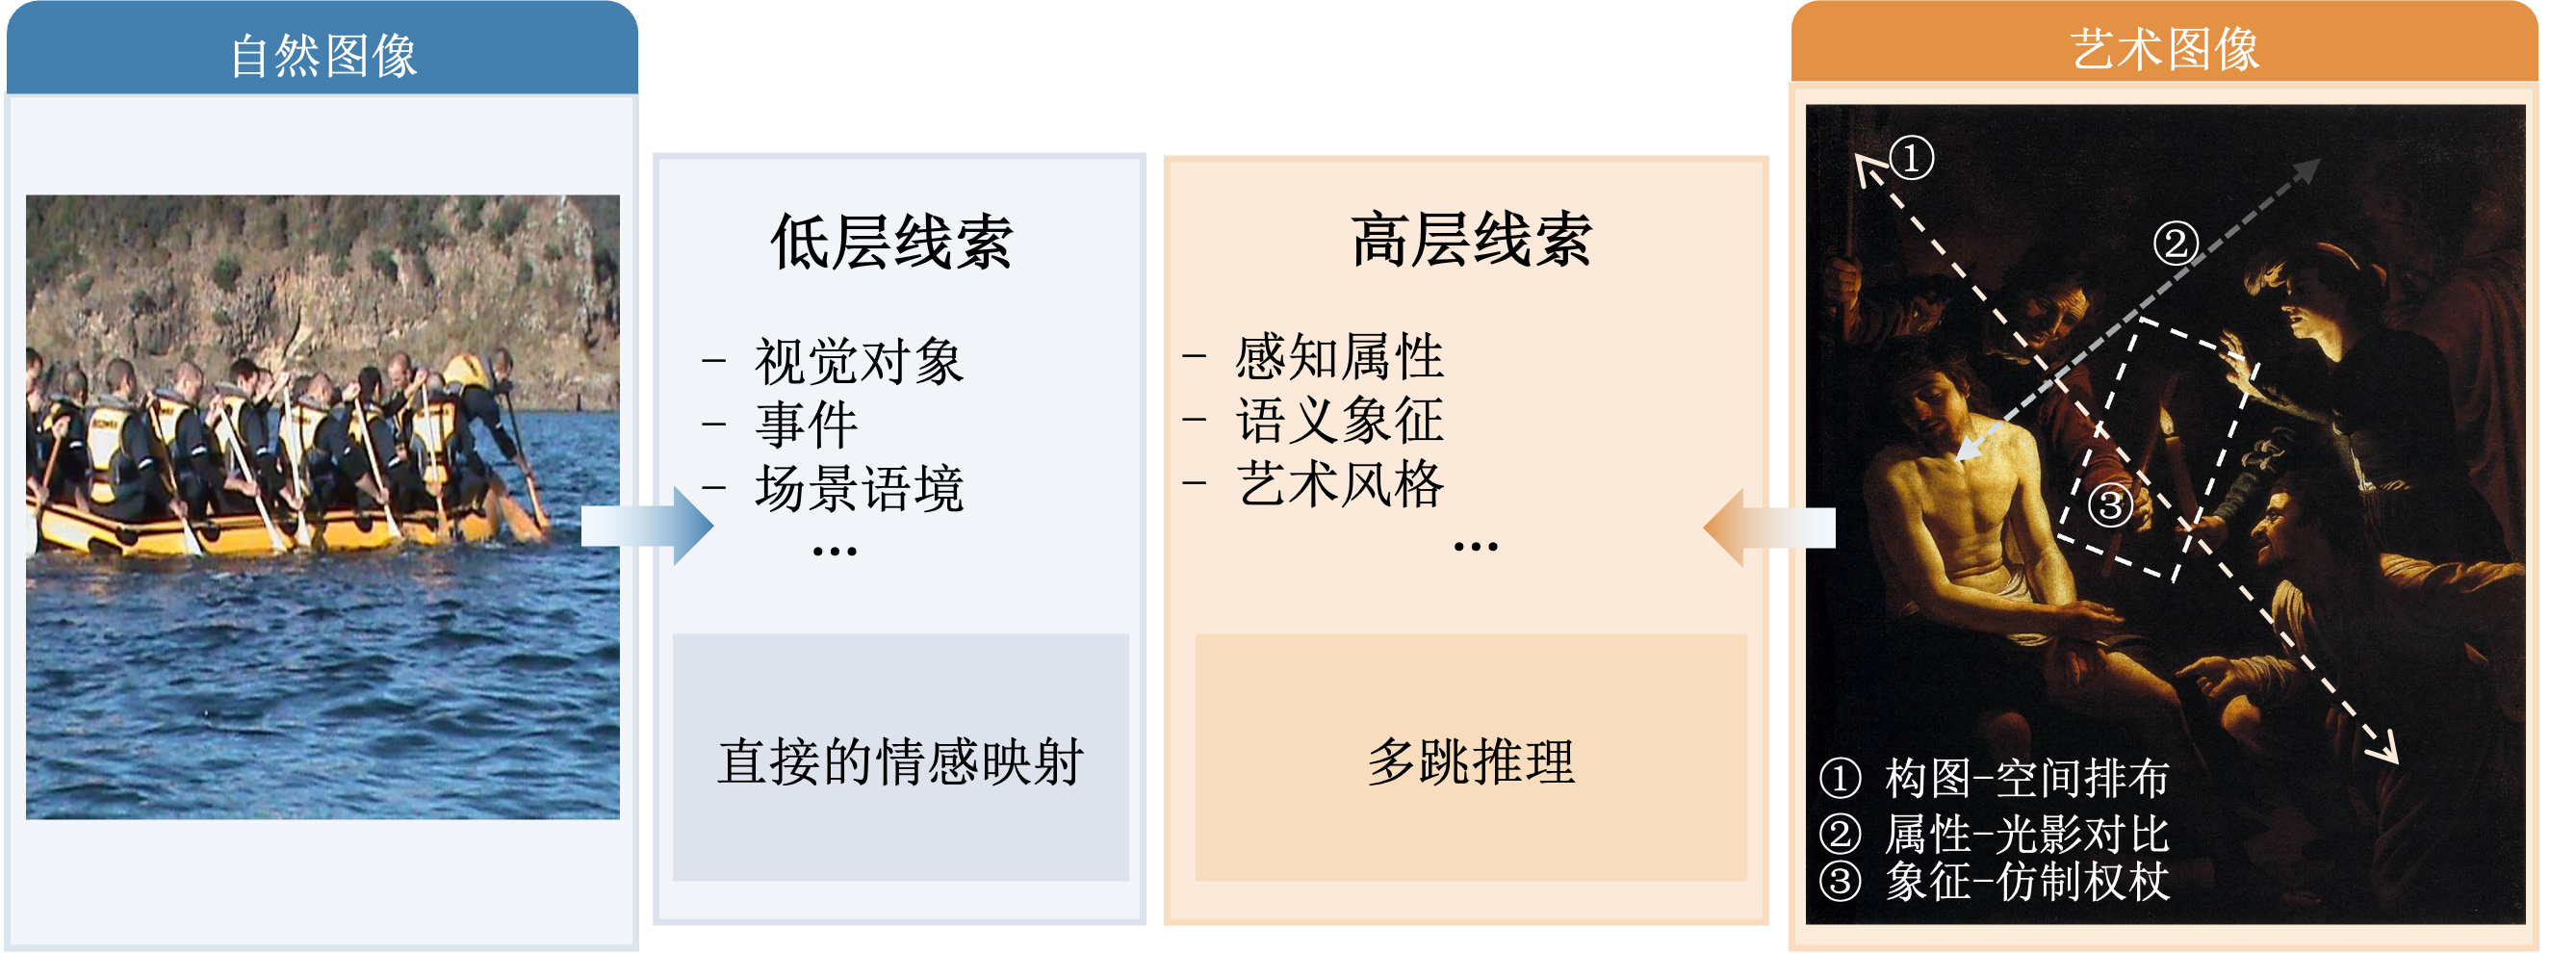
\includegraphics[width=0.92\textwidth]{figures/aerbench/moti.png}
    \bicaption[fig:chap5_main_comparison]{}{自然图像与艺术图像情感推理的差异：从显式实体线索到隐式形式线索的跨越}{Fig.}{Comparison between ordinary image emotion reasoning and art image emotion reasoning, highlighting the shift from explicit cues to implicit aesthetic cues}
\end{figure}

AER-Bench 通过以下方式实现上述评测目标：在数据层面，从覆盖八类艺术风格的 2,058 件作品中构建具有风格多样性的图像集合；在标注层面，采用 GPT-4o~\cite{achiam2023gpt} 辅助的结构化标注框架，结合 CLIP~\cite{radford2021learning} 相似度过滤与多轮人工核验，确保标注的内部一致性；在任务层面，采用固定模板而非自由提示生成评测题目，并通过单图与双图两种设置同时考察模型的图像内推理能力与图像间关系推理能力。基准最终产出 24,792 个单图任务与 9,999 个配对任务；在模型层面，覆盖 4 个闭源与 10 个开源 MLLM，合计 14 个代表性模型的系统评测，从而支撑跨模型、跨设置的能力对比与失败模式分析。

本章的主要贡献可总结为以下三点：
\begin{enumerate}
    \item AER-Bench 多层级诊断基准：构建首个面向艺术情感推理的多层级诊断型基准，通过结构化的“感知—情感—推理—描述”四级标注体系对艺术情感理解过程进行显式分解，并据此生成可重复、可对齐的评测任务，覆盖 2,058 件作品、24,792 个单图任务与 9,999 个配对任务。
    \item 统一评测协议：融合确定性度量与基于评分的语义评判，将客观题与开放式题置于同一评测框架下，覆盖感知单选、情感排序、评分、配对推理与开放式描述多种任务形式，同时支撑单图与双图两种设置的能力诊断。
    \item 模型系统评测与瓶颈揭示：在 14 个代表性 MLLM 上系统评测，揭示当前 MLLM 在艺术情感理解上的核心瓶颈——能够生成看似合理的情感标签或流畅的情感描述，但难以将这些输出锚定到具体的感知线索、上下文证据与表达模式上，体现出在“基于证据的解释”层面的系统性能力缺口。
\end{enumerate}

\section{面向图像情感语义的基准设计与评测}

\label{sec:chap5_benchmark_design}

AER-Bench 将艺术情感理解形式化为一个由低到高的四级能力体系：感知维度层（Perception）刻画从低层视觉形式到高层情感的中介证据，情感与 VAD 层（Emotion \& VAD）刻画情感判断本身，推理层（Reasoning）刻画从证据到情感的解释过程，描述层（Description）刻画对作品整体情感氛围的综合表达。这一四级体系直接对应数据标注与任务生成的层级结构，使模型的能力缺陷能够被精确定位到具体层级。

\begin{figure}[!htbp]
    \centering
    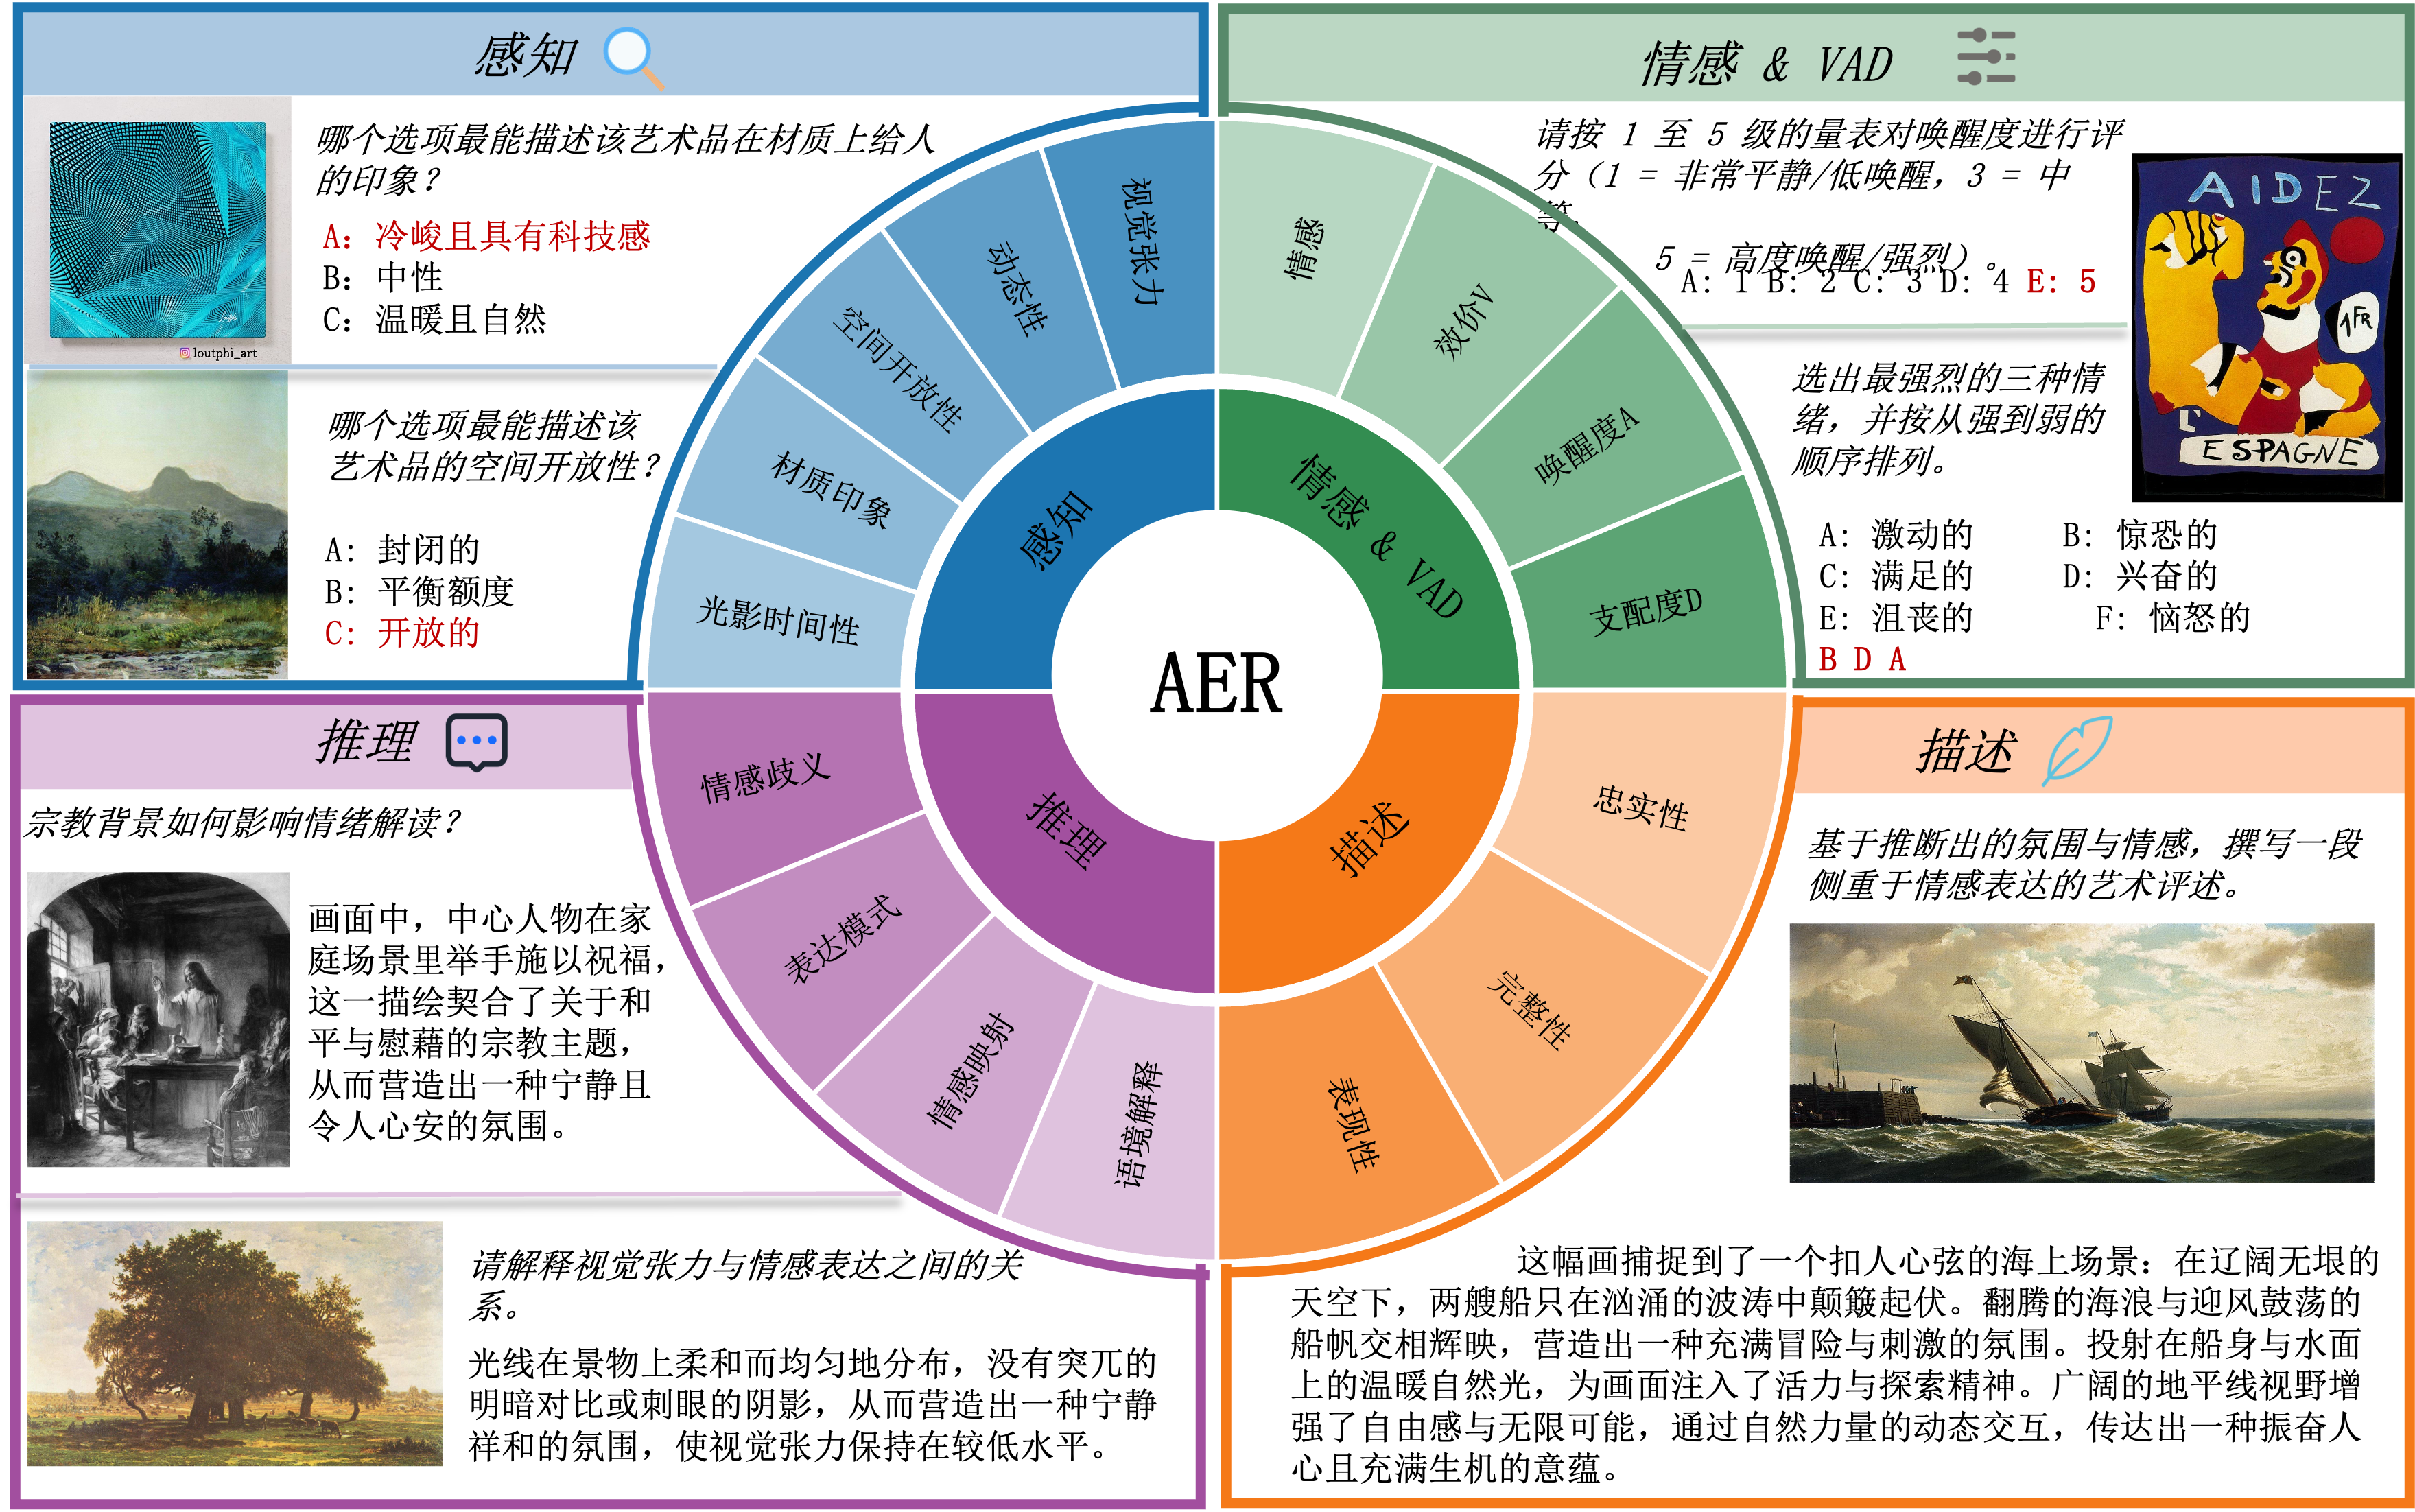
\includegraphics[width=0.95\textwidth]{figures/aerbench/main.png}
    \bicaption[fig:chap5_comp]{}{AER-Bench 评测体系总览}{Fig.}{Overview of the AER-Bench design}
\end{figure}

\subsection{多维语义层级建模}

\label{sec:chap5_four_layer_representation}

本节按由低到高的顺序，将艺术情感推理过程形式化为感知维度、情感与 VAD、证据锚定推理与综合氛围描述四个层级，并使每层既可独立评测、又可与上一层形成依赖关系，从而支撑对模型能力的层级化诊断。

感知维度层作为低层视觉形式通往高层情感的中介证据，借鉴 Arnheim《Art and Visual Perception》中关于“形式—情感关系”的论述~\cite{arnheim1954art}与 Zhao 等人提出的“艺术原则特征”~\cite{zhao2014exploring}，将艺术作品的形式特征操作化为视觉张力（visual tension）、动态性（dynamism）、空间开放性（spatial openness）、材质印象（material impression）与光照时间性（light temporality）五个可标注维度；相较于纯粹基于色彩、纹理等低层视觉元素的特征~\cite{lu2012shape}，感知维度更接近艺术创作与艺术评论所使用的描述语言，能够同时服务于标注与评测。

情感与 VAD 层在感知维度所揭示的形式证据之上，刻画模型对作品情感状态的直接判断。离散标签方面，采用 12 个共享情感词（兴奋aroused、激动excited、快乐happy、悲伤sad、无聊bored、疲惫tired、惊恐alarmed、恼怒annoyed、沮丧frustrated、高兴glad、满足contentment、平静calm）构成的有限集合，覆盖从高唤醒度到低唤醒度、从正效价到负效价的完整情感谱系~\cite{warriner2013norms,eemobench2025}；连续维度方面，采用情感心理学中广泛使用的 效价--唤醒度--支配度（VAD）三维评分~\cite{warriner2013norms}，三维均采用 1--5 量表，并与 Warriner 等发布的 13,915 词英语 VAD 词典在取值范围与情感语义上保持一致，便于在词级别进行跨数据集的语义对齐，三个维度在 1--5 量表上的锚点定义见附录~\ref{app:aerbench_supplement}。离散标签保证情感判断的可解释性，VAD 维度保证与情感心理学已有范式的可对接性，二者共同支撑模型在情感粒度上的多尺度能力评测。

证据锚定推理层进一步评估模型能否将上述情感判断锚定到具体的视觉证据与上下文线索上，而非仅给出情感标签本身。借鉴 Panofsky 的图像学分析框架~\cite{panofskyiconography}与艺术评论中“形式—语境—意图”的分析路径，AER-Bench 将推理进一步细分为四个子维度：（1）情感映射（affective mapping）评估模型能否显式说明特定感知维度如何支撑其情感判断；（2）语境（context）评估模型在涉及历史、文化、宗教、政治或符号背景时能否恰当地调整情感解释；（3）多义性（ambiguity）评估模型在多实体、主体—背景或形式—内容冲突情境下能否辨识与权衡；（4）隐性表达（implicit impression）评估模型能否识别作品以直接、间接或混合方式传达情感。

综合氛围描述层在前三个层级之上，评估模型对作品整体情感氛围的综合表达能力，要求描述同时覆盖表现性（expressiveness，是否流畅且富有情感表现力）、完整性（completeness，是否覆盖主要情感氛围与关键描述要点）与忠实性（faithfulness，是否与作品视觉证据一致、无凭空捏造）三个属性，避免出现“流畅但无证据”式的情感短语堆砌；该三元评估基准与开放词汇描述生成领域的可解释性研究~\cite{emoart2025,achlioptas2021artemis}保持一致。四个层级共同构成从“视觉证据”到“情感判断”再到“证据化解释”的完整评测链条，使模型在每一抽象层级的缺陷都能被精确定位。这一层级化结构直接体现在基准的构造流程中：结构化标注经由模板化题合成被实例化为评测任务，使能力缺陷能够被定位到具体层级，如图~\ref{fig:chap5_data_build}所示。

\begin{figure}[!htbp]
    \centering
    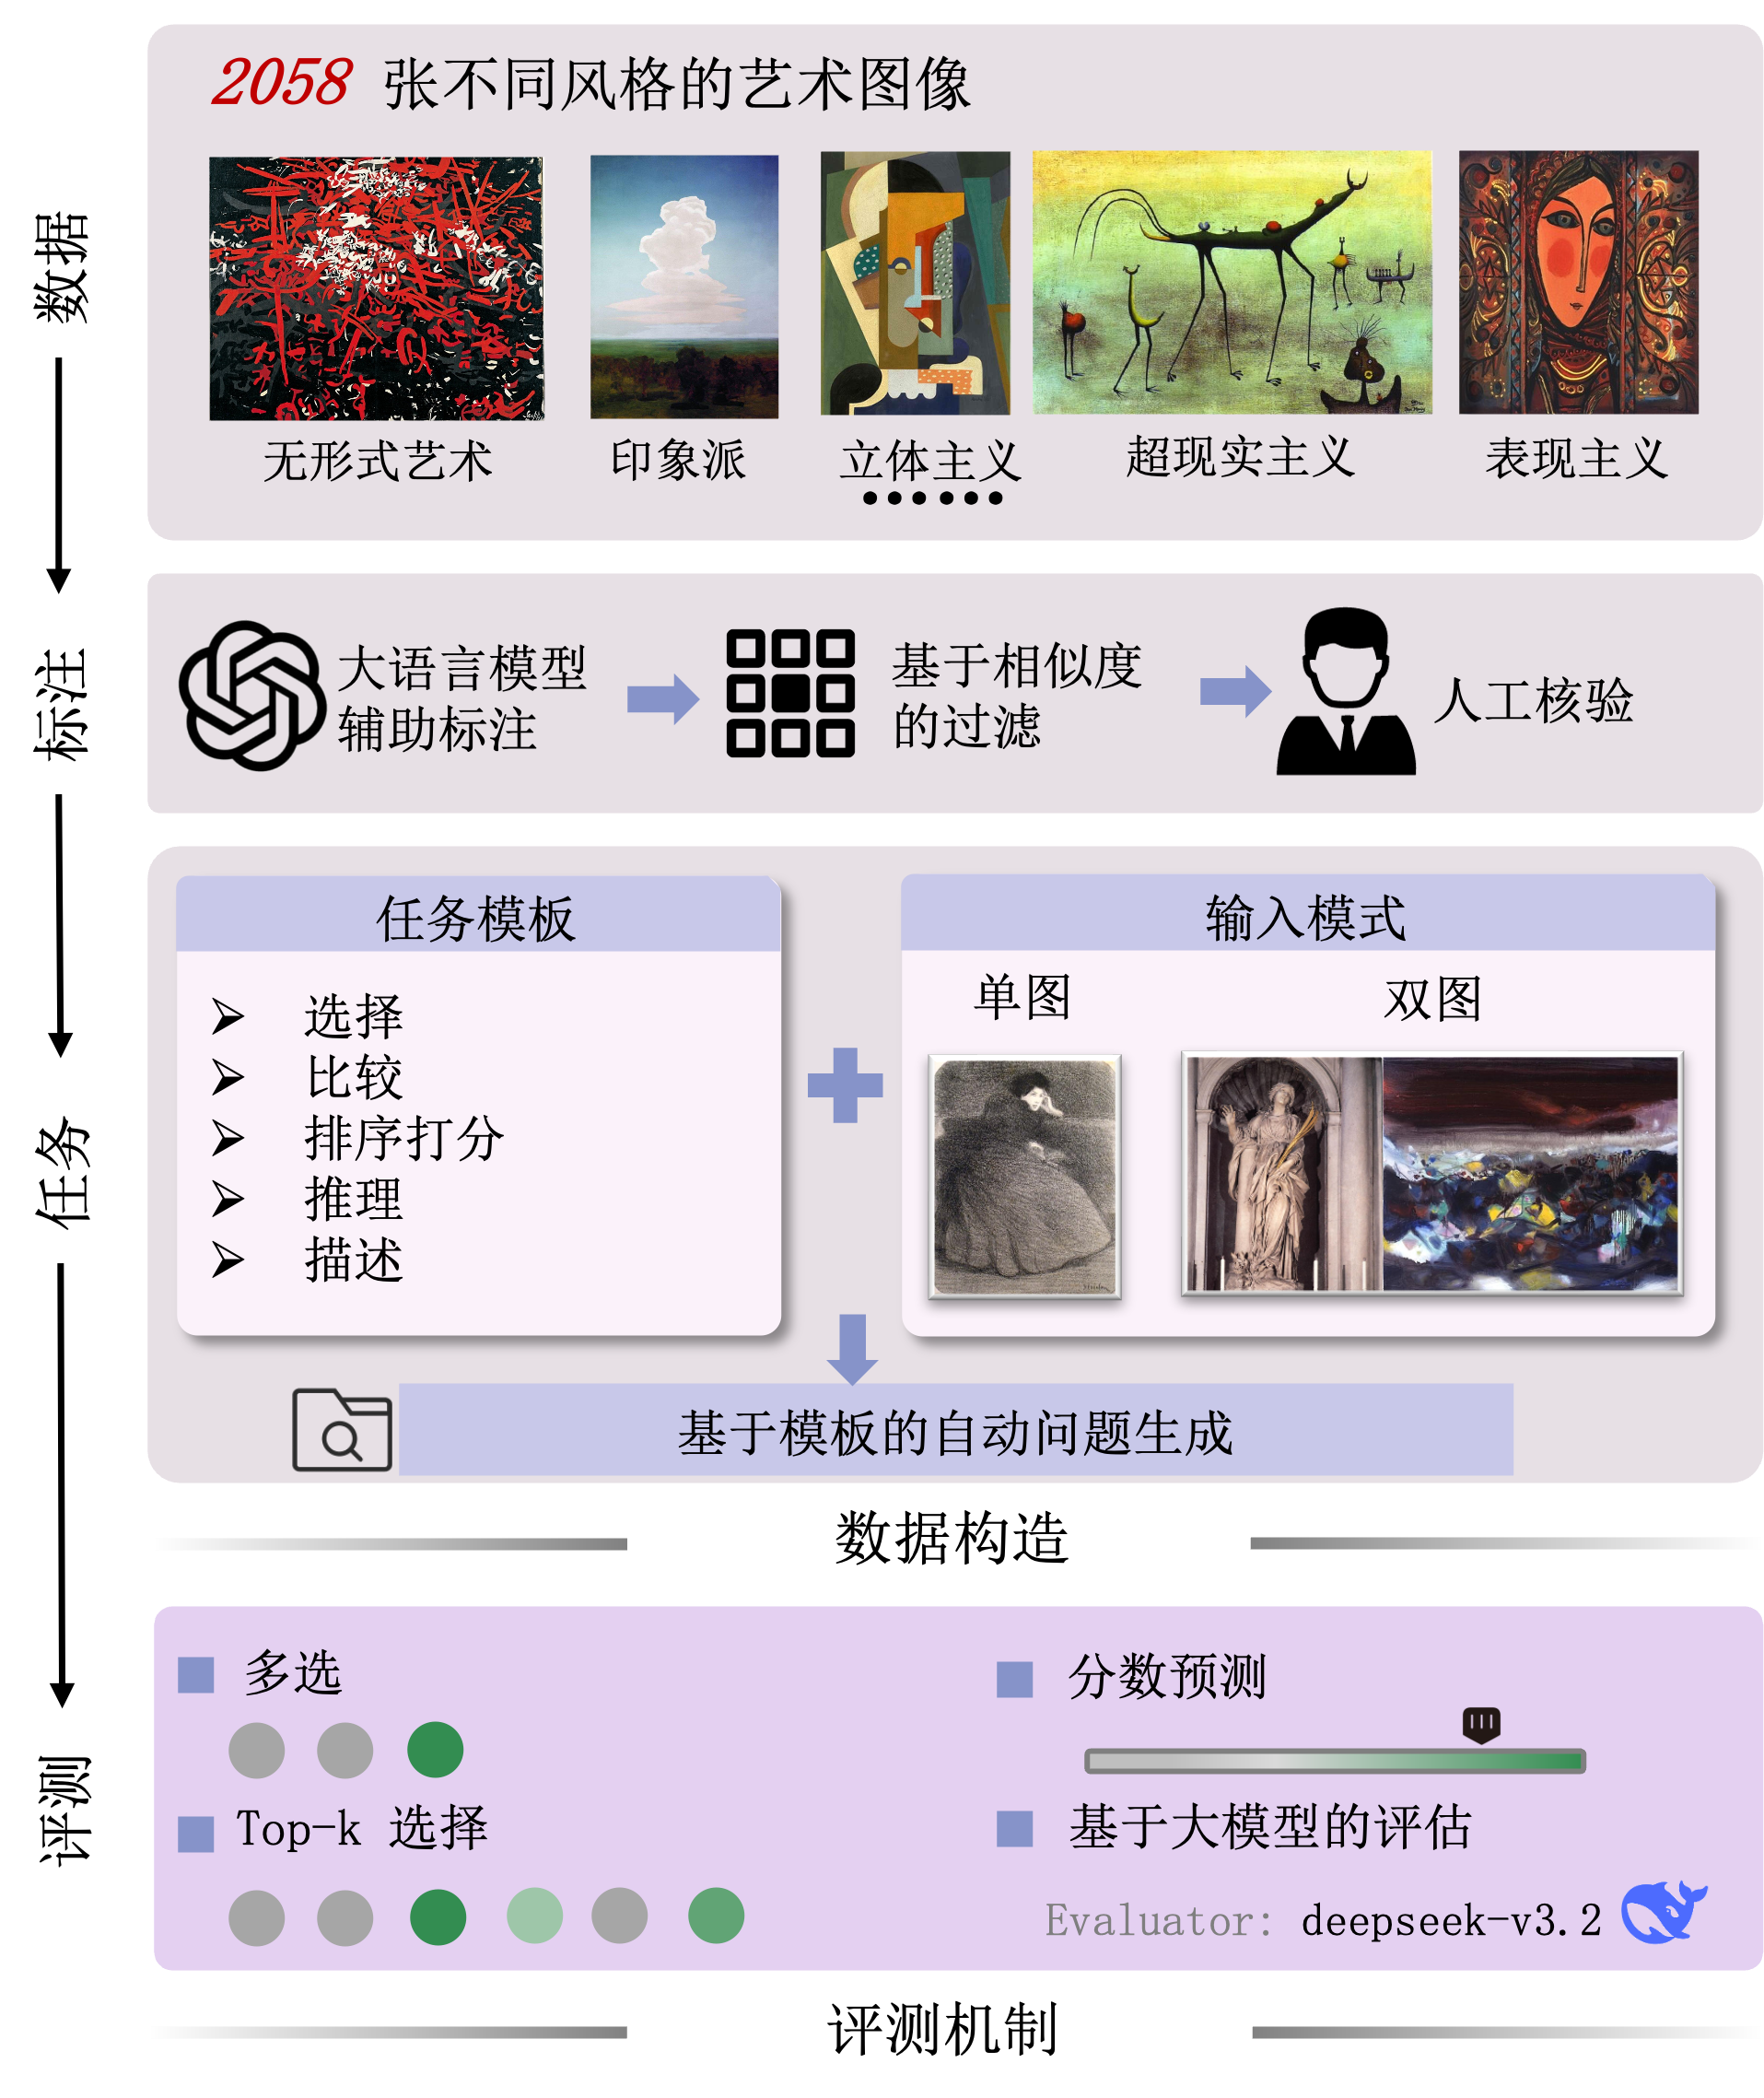
\includegraphics[width=0.65\textwidth]{figures/aerbench/data_build.png}
    \bicaption[fig:chap5_data_build]{}{AER-Bench 构造流程总览}{Fig.}{Overview of the benchmark construction pipeline}
\end{figure}

\subsection{数据质量控制与系统评测}

\label{sec:chap5_data_pipeline}

为保证视觉与风格多样性，AER-Bench 的源图像采集自 WikiArt\footnote{\url{https://www.wikiart.org/}}，这是一个覆盖从文艺复兴至当代抽象艺术的大规模在线艺术作品集合。考虑到艺术情感常常由作品的形式结构、绘画风格、象征内容与观者诠释共同决定，而非由单一显式对象承载，WikiArt 的风格多样性天然契合本基准对情感表达异质性的需求。采样过程按以下顺序执行：首先进行初始检索，在 WikiArt 上按多个时期与流派进行广泛候选抓取，最大化风格与主题覆盖；随后进行风格分层，将候选作品归入八大风格家族——现实主义、印象主义、表现主义、抽象艺术、超现实主义、象征主义、当代艺术、其他，并按比例分层采样，避免对单一艺术传统的过表征，确保下游任务不会被某一熟识的美学惯例系统性偏置；最后采用相似度过滤去除近重复样本。经过上述筛选，最终保留 2,058 件作品作为基准源集合。

AER-Bench 采用以 GPT-4o~\cite{achiam2023gpt} 为辅助的结构化标注策略：标注提示要求模型按照预定义的 JSON 模式，针对每件作品同时输出五维感知评分、情感 Top-3 与 VAD 三维、情感描述与基于证据的推理四个层级的标注，其关键指令与取值约束汇总于表~\ref{tab:chap5_prompt_summary}；为保证大规模标注的可重复性与可恢复性，标注管线引入了系统化的错误处理与断点续传机制。标注质量通过多层过滤与人工核验共同保证：
在自动过滤方面，针对单选感知题，使用 CLIP（ViT-L-14）~\cite{radford2021learning} 计算图像—选项对的相似度，仅保留真值选项在 CLIP 相似度上具有显著优势的样本，从而去除视觉不一致或歧义过大的实例；针对配对题，使用 GPT-4o 对同一对图像进行独立复核，将分歧样本对齐到模型判断，并仅保留确定且置信度足够的样本。
在人工核验方面，从全部标注中按任务类型分层随机抽样，由三位具备视觉艺术与多模态评估背景的标注员独立核验。相关结果位于表~\ref{tab:chap5_llm_judge}:标注一致性（Krippendorff's $\alpha$）超过 0.68，调整一致率（adjusted agreement， Adj.Agr）达 95.2\%，平均得分 0.79（归一化至 [0,1] 区间），证明标注能够被领域专家接受；核验的设计与评分细则见附录~\ref{app:human_verification}。


\begin{table}[!htbp]
    \bicaption[tab:chap5_llm_judge]{}{AER-Bench LLM 评判与人类专家一致性核验}{Table}{Validation of AER-Bench LLM judge against human experts}
    \vspace{0.5em}\centering\wuhao
    \setlength{\tabcolsep}{4pt}
    \begin{tabular}{lrccccc}
    \toprule
    \multirow{2}{*}{任务} & \multirow{2}{*}{N} &
    \multicolumn{3}{c}{\textit{标注核验}} &
    \multicolumn{2}{c}{\textit{LLM 评判核验}} \\
    \cmidrule(lr){3-5}\cmidrule(l){6-7}
     & &
    Hum.-$\alpha$ & Adj.\ Agr.\ (\%) & 平均 & LLM--Hum.\ $\kappa_w$ & Self-$\alpha$ \\
    \midrule
    单图推理 & 120 & 0.74 & 96.8 & 0.89 & 0.69 & 0.88 \\
    配对推理 & 120 & 0.69 & 94.3 & 0.77 & 0.58 & 0.85 \\
    情感描述 & 120 & 0.61 & 92.1 & 0.72 & 0.53 & 0.83 \\
    \midrule
    整体 & 360 & 0.68 & 95.2 & 0.79 & 0.60 & 0.86 \\
    \bottomrule
    \end{tabular}
\end{table}

\begin{table}[!htbp]
    \centering
    \bicaption[tab:chap5_prompt_summary]{}{标注与开放式评测所用提示词要点汇总}{Table}{Summary of prompts used for annotation and open-ended evaluation}
    \vspace{0.5em}\centering\wuhao
    \setlength{\tabcolsep}{5pt}
    \renewcommand{\arraystretch}{1.15}
    \begin{tabularx}{\textwidth}{@{}>{\raggedright\arraybackslash}p{0.17\textwidth}>{\raggedright\arraybackslash}X@{}}
    \toprule
    提示词 & 关键指令与评分细则 \\
    \midrule
    标注提示词 & 要求模型作为艺术情感分析专家，针对给定图像返回且仅返回一个严格遵循既定 JSON 模式的标注对象。标注规则为：$\mathcal{O}_{\text{per}}$ 为五维感知画像，$\mathcal{O}_{\text{emo}}$ 为与 $\mathcal{O}_{\text{per}}$ 一致的情感标签与 VAD 取值，$\mathcal{O}_{\text{des}}$ 为聚焦情感的表述，$\mathcal{O}_{\text{rea}}$ 为基于证据的简明推理；$\mathcal{O}_{\text{des}}$ 与 $\mathcal{O}_{\text{rea}}$ 中的每一项关键论断都必须给出具体的视觉证据锚点。 \\
    \midrule
    推理评判提示词 & 要求模型作为艺术图像情感推理专家，在给定任务上下文、被评响应与参考答案后进行评分。评分细则为：2 分表示完整、准确且切题；1 分表示部分正确或切题，但遗漏重要细节或存在轻微偏差；0 分表示无效、不切题或大体错误。评判关注语义正确性与推理质量，而不要求字面表述一致。 \\
    \midrule
    描述评判提示词 & 要求模型作为艺术作品情感描述评判专家，在表现性、完整性与忠实性三个维度上评价被评响应。评分细则为：2 分表示三个维度均表现良好或几乎均表现良好；1 分表示部分正确，但一个或多个维度偏弱；0 分表示多数维度表现差、不切题或不忠实。评判同样以语义而非字面表述为准。 \\
    \bottomrule
    \end{tabularx}
\end{table}

标注对象划分、字段级模式与取值约束由附录~\ref{app:aerbench_supplement}给出，本节重点关注与评测直接相关的指标与协议。

为保证可重复性，题生成采用固定模板而非自由提示：模板化合成在显著降低题面语言学方差的同时，保留了标注本身所编码的推理难度——基准考察的是模型能否从视觉与语义证据推断情感关系，而非能否适应不可控的提示措辞。对每条有效标注实例，AER-Bench 合成以下五类受控任务：感知维度单选，即从五个感知维度分别构造单选感知题，模型输出归一化为选项值，使用精确匹配准确率评分；情感 Top-3 排序，从共享 12 词情感池中抽取 6 个候选，含真值 top-3 与 3 个 distractor，要求模型给出排序，使用 Hit@3 与 NDCG@3~\cite{NDCG} 的加权得分；配对题构造配对感知、配对 VAD 与配对推理三类，统一为左右单选格式；开放式推理题，要求模型给出基于证据的解释，使用基于 rubric 的语义评判；开放式描述题，要求模型给出对作品整体情感氛围的描述，同样使用基于 rubric 的语义评判。上述任务在图~\ref{fig:chap5_data_build}所示的构造流程中统一由结构化标注实例化得到，并被分配到两种互补的评测设置：单图设置考察模型能否从作品自身的内在组织中推断情感意义，配对设置则考察这种解释在比较性视觉语境下是否保持稳定。由于既有研究表明艺术照片的情感解读会系统性地受到邻近图像的影响~\cite{reymond2025pictorial}，配对任务提供了对关系敏感性的更强检验，并可降低模型仅依赖图像内在先验的倾向。表~\ref{tab:chap5_data_stats} 给出了最终数据集的规模与任务组织。

\begin{table}[!htbp]
    \bicaption[tab:chap5_data_stats]{}{AER-Bench 数据集统计与任务组织}{Table}{Dataset statistics and task organization of AER-Bench}
    \vspace{0.5em}\centering\wuhao
    \setlength{\tabcolsep}{4pt}
    \begin{tabularx}{\linewidth}{@{}p{0.20\linewidth}XrX@{}}
    \toprule
    \textbf{类别} & \textbf{子集} & \textbf{数量} & \textbf{说明} \\
    \midrule
    样本规模
        & 艺术作品 & 2,058 & 经筛选的细粒度艺术图像集合 \\
    \midrule
    \multirow{5}{=}{闭合题}
        & 单图感知 & 3,946 & 感知维度单选 \\
        & 单图情感与 VAD & 8,232 & 情感排序与 VAD 评分 \\
        & 配对感知 & 3,651 & 左右单选 \\
        & 配对 VAD & 3,544 & 左右单选 \\
        & 配对推理 & 2,804 & 左右单选 \\
    \midrule
    \multirow{2}{=}{开放式}
        & 单图推理 & 10,556 & 自由文本解释 \\
        & 单图描述 & 2,058 & 自由文本情感描述 \\
    \bottomrule
    \end{tabularx}
\end{table}

\subsection{评测指标与跨基准定位}

\label{sec:chap5_metrics}

闭合题采用精确匹配准确率或加权排序得分。对于情感 Top-3 排序任务，AER-Bench 采用 Hit@3 与 NDCG@3 的加权和作为主要评分。Hit@3 衡量预测 Top-3 与参考 Top-3 集合的无序重合程度：
\begin{equation}
\mathrm{Hit@3}=\frac{|\hat{Y}_{1:3}\cap Y_{1:3}|}{3},
\label{eq:chap5_hit3}
\end{equation}
其中 $\hat{Y}_{1:3}$ 与 $Y_{1:3}$ 分别为预测与参考的 Top-3 情感集合。NDCG@3 则在此基础上进一步刻画排序质量：设 $r_k$ 为位置 $k$ 处的参考相关度（参考排名第 1、2、3 位对应相关度 3、2、1，其余为 0），$\hat{y}_k$ 与 $y_k$ 分别为预测与理想情况下位置 $k$ 的情感，则：
\begin{equation}
\mathrm{NDCG@3}=\frac{\sum_{k=1}^{3}\frac{r(\hat{y}_k)}{\log_2(k+1)}}{\sum_{k=1}^{3}\frac{r(y_k)}{\log_2(k+1)}}.
\label{eq:chap5_ndcg3}
\end{equation}

最终的情感排序得分取两者的加权和（$\alpha_{\text{top3}}=0.5$）：
\begin{equation}
S_{\text{Top3}}=\alpha_{\text{top3}}\cdot\mathrm{Hit@3}+(1-\alpha_{\text{top3}})\cdot\mathrm{NDCG@3}.
\label{eq:chap5_stop3}
\end{equation}

VAD 题采用对中性点方向敏感的均值情感得分（取值区间 [0,1]）。具体地，设模型对某一 VAD 维度的预测为 $\hat{v}$、参考值为 $v$，该项得分为：
\begin{equation}
S_{\text{VAD}}(\hat{v},v)=\max\left(0,\frac{100-20|\hat{v}-v|-p_{\text{pen}}}{100}\right),
\label{eq:chap5_svad}
\end{equation}
其中 $p_{\text{pen}}=15$ 当预测与参考落在中性点（值为 3）两侧，$p_{\text{pen}}=5$ 当其一为中性而另一为非中性；该设计对跨越情感极性的预测错误施加更重的惩罚，避免模型通过“全部预测为中性”获得表面可观的分数。

开放式题推理与描述采用基于 rubric 的语义评判：对每个响应，由评判模型GPT-4o按照预定义的评分细则输出 0--2 的整数分，推理题与描述题分别对应表~\ref{tab:chap5_prompt_summary}中的推理评判提示词与描述评判提示词。评分关注语义正确性而非字面一致，因此合理改写不会被错判。为检验 LLM 评判的可信度，AER-Bench 在 360 个响应（每类 120 条）上将其与三位人类专家的评判进行对比，结果如表~\ref{tab:chap5_llm_judge}所示。LLM 评判与专家中位分数的二次加权 Cohen's $\kappa_w$ 达到 0.60；在同一批响应上重复评判五次，整体自我一致性 $\alpha=0.86$；LLM--人类一致度序列$\kappa_w$ （0.69、0.58、0.53）与标注平均得分序列（0.89、0.77、0.72）平行递减，表明评判的任务难度差异主要反映了各任务固有的判别难度，而非评判者的偶发偏好。据此可以认为模型评判在语义正确性、相关性、推理质量与关键证据覆盖四个维度上足以替代人工专家承担开放式题的常规评判。

表~\ref{tab:chap5_dataset_compare} 将 AER-Bench 与 ArtEmis~\cite{achlioptas2021artemis}、EmoSet~\cite{yang2023emoset}、EmoArt~\cite{emoart2025}、EEmo-Bench~\cite{eemobench2025} 四类代表性视觉情感资源在领域、完整 VAD、情感描述、结构化推理与双图设置等维度上做了横向对比。可以看到：AER-Bench 是唯一同时具备“艺术领域 + 完整 VAD + 情感描述 + 结构化推理 + 双图设置”的基准，这使得它能够同时诊断模型在单图情感理解与配对情感校准两个层面上的能力差距。

\begin{table*}[!htbp]
    \centering
    \bicaption[tab:chap5_dataset_compare]{}{代表性视觉情感数据集/基准的对比}{Table}{Comparison with representative visual emotion datasets and benchmarks}
    \vspace{0.5em}\wuhao
    \setlength{\tabcolsep}{6pt}
    \begin{tabularx}{.85\textwidth}{lccc>{\centering}Xc}
        \toprule
         & 领域 & 完整 VAD & 情感描述 & 推理 & 双图 \\
        \midrule
        ArtEmis~\cite{achlioptas2021artemis} & 艺术 & $\times$ & \checkmark & 开放式 & $\times$ \\
        EmoSet~\cite{yang2023emoset} & 照片 & $\times$ & $\times$ & $\times$ & $\times$ \\
        EmoArt~\cite{emoart2025} & 艺术 & 仅 A/V & \checkmark & $\times$ & $\times$ \\
        EEmo-Bench~\cite{eemobench2025} & 照片 & \checkmark & \checkmark & 开放式 & \checkmark \\
        AER-Bench & 艺术 & \checkmark & \checkmark & 结构化 & \checkmark \\
        \bottomrule
    \end{tabularx}
\end{table*}




% 本节从基准设计的内禀结构出发，给出了 AER-Bench 的完整方案。在能力维度上，基准通过感知维度—情感与 VAD—推理—描述的四级递进体系，将艺术情感理解显式分解为可独立评测的子能力；在数据管线上，通过 WikiArt 多风格采样、GPT-4o 辅助结构化标注与 CLIP 相似度过滤三层保障，构建了 2,058 件作品、24,792 个单图任务与 9,999 个配对任务的高质量基准；在评测协议上，通过客观题（Hit@3/NDCG@3/$S_{\text{VAD}}$）与基于 rubric 的开放式语义评判的统一框架，在保证可解释性的同时支持对开放式推理与描述的细粒度评估；在横向定位上，AER-Bench 是首个同时具备艺术领域、完整 VAD、情感描述、结构化推理与双图设置的基准，填补了当前艺术情感评测的空白。整体而言，本节为后续模型评测提供了结构清晰、协议统一、可重复对齐的评测基础。
\FloatBarrier

\section{数据与实验分析}

\label{sec:chap5_analysis_findings}

    \subsection{数据统计分析}

\label{sec:chap5_stat_profile}

图~\ref{fig:chap5_emotion_distribution} 给出了 AER-Bench 中 Top-3 情感标签的分布。整体来看，情感分布呈现向“低唤醒、正向”情感显著倾斜的特征：calm 与 contentment 在 Top-3 中占据主导地位，而 alarmed、frustrated、annoyed 等高唤醒负向情感的出现频次明显较少。这一偏态与 Berlyne 提出的“arousal potential”理论一致——观者倾向于偏好具有“中等复杂度”且“结构平衡”的刺激：过于单一会失去兴趣，过于刺激则会引发负向情感；这种平衡既能维持观者的注意力，又不会造成认知过载，因而更容易引发心理平衡与审美愉悦状态。该分布形态意味着：仅靠“总是预测为最常见情感”的退化策略在 AER-Bench 上无法取得显著优势，模型必须学会识别艺术作品所特有的中介线索。

\begin{figure}[!htbp]
    \centering
    \includegraphics[width=0.85\textwidth]{papers/AER-Bench/figures/emotion_distribution.pdf}
    \bicaption[fig:chap5_emotion_distribution]{}{AER-Bench 中 Top-3 情感标签的分布}{Fig.}{Distribution of top-3 emotion labels in the benchmark}
\end{figure}

为检验 AER-Bench 中离散的 Top-1 情感标签与连续的 VAD 三维之间是否保持系统性共变，对 12 个情感类别在三个 VAD 维度上分别执行 Kruskal--Wallis 秩和检验。设样本量 $n=2{,}058$，情感类别数 $K_{\text{emo}}=12$，检验统计量 $H_{\text{KW}}$、效应量 $\epsilon^2$ 与渐近 $p$ 值列于表~\ref{tab:chap5_emotion_vad_consistency}。三个维度的检验均给出高度显著的 $p$ 值（$<10^{-123}$），表明在每个 VAD 维度上，情感类别间的分布差异均显著大于随机波动。其中 $\epsilon^2$由情感分组解释的 VAD 变异占比在效价与唤醒度上达到“中—大”效应量阈值（0.06/0.14），支配度上也达到的“中等偏大”水平。该结果一方面验证了 AER-Bench 在标注层面保持了离散与连续两种情感表征之间的内部一致性，另一方面也为评测提供了双重锚点：模型既需要命中正确的离散情感，又需要给出方向一致的 VAD 评分。

\begin{table}[!htbp]
    \centering
    \wuhao
    \setlength{\tabcolsep}{6pt}
    \begin{minipage}[t]{0.49\linewidth}
        \centering
        \bicaption[tab:chap5_emotion_vad_consistency]{}{Top-1 情感标签与 VAD 评分内部一致性}{Table}{Internal consistency between top-1 emotion labels and VAD scores}
        \vspace{0.3em}
        \begin{tabular}{lccc}
        \toprule
        维度 & $H_{\text{KW}}$ & $\epsilon^2$ & $p$ \\
        \midrule
        效价 & 961.24 & 0.464 & $<10^{-198}$ \\
        唤醒度 & 1314.42 & 0.637 & $<10^{-274}$ \\
        支配度 & 611.46 & 0.293 & $<10^{-123}$ \\
        \bottomrule
        \end{tabular}
    \end{minipage}
    \hfill
    \begin{minipage}[t]{0.49\linewidth}
        \centering
        \bicaption[tab:chap5_cramersv]{}{感知维度与情感标签的关联强度}{Table}{Association between perception dimension values and emotion labels}
        \vspace{0.3em}
        \begin{tabular}{lc}
        \toprule
        感知维度 & Cramer's V \\
        \midrule
        视觉张力 & \textbf{0.5310} \\
        动态性 & 0.4989 \\
        空间开放性 & 0.2166 \\
        材质印象 & 0.2557 \\
        光照时间性 & 0.2259 \\
        \bottomrule
        \end{tabular}
    \end{minipage}
\end{table}


\begin{figure}[!htbp]
    \centering
    \includegraphics[width=0.75\textwidth]{papers/AER-Bench/figures/representative_trend_matrix_set5.pdf}
    \bicaption[fig:chap5_perception_examples]{}{感知维度层的代表性作品示例}{Fig.}{Representative artworks illustrating trend values across the five perception dimensions}
\end{figure}

\begin{figure}[!htbp]
    \centering
    \includegraphics[width=0.92\textwidth]{papers/AER-Bench/figures/sdim_emotion_cooccurrence_overview.pdf}
    \bicaption[fig:chap5_perception_emotion_cooccurrence]{}{感知维度与情感标签之间的共现结构总览}{Fig.}{Overview of the co-occurrence structure between perception dimensions and emotion labels}
\end{figure}
图~\ref{fig:chap5_perception_examples} 与图~\ref{fig:chap5_perception_emotion_cooccurrence} 分别给出感知维度层的代表性作品示例与共现结构总览。为定量刻画五个感知维度与情感标签之间的关联强度，进一步使用 Cramer's V（列联系数 $V$）~\cite{cramer1999mathematical}计算每一维度对情感标签的条件分布的相关性，结果列于表~\ref{tab:chap5_cramersv}。其中视觉张力与情感标签的相关性最强（$V=0.5310$），动态性（dynamism）次之（$V=0.4989$），空间开放性、材质印象、光照时间性则相对较弱（$V\in[0.21,0.26]$）。


这一排序揭示了艺术情感判读中两条相对独立的中介线索：（1）以视觉张力—动态性为核心的结构性线索，构成了与情感标签最强、最稳定的对应关系——视觉张力越低，越倾向于被解读为 calm 与 contentment；视觉张力越高，越倾向于被解读为 alarmed、frustrated、aroused；动态性同样形成了“静—动”轴线，静或缓变的构图更多与 calm 类情感关联，强动态性与高唤醒情感关联。（2）以空间开放性、材质印象、光照时间性为辅助的修饰性线索，它们对情感条件分布的影响相对弱但仍具有可解释的偏移——这些维度更多承担“作品风格与氛围修饰”的角色，而非情感判读的支配性证据。

\FloatBarrier

\subsection{实验结果对比}

\label{sec:chap5_main_results}

本节在 AER-Bench 上对 14 个代表性 MLLM 进行系统评测，覆盖 4 个闭源模型（GPT-5.4、Qwen-VL-Max~\cite{bai2023qwen}、Gemini-2.5-Pro 与 Gemini-2.5-Flash~\cite{comanici2025gemini}）与 10 个开源/开放权重的 MLLM（Qwen3-VL-8B~\cite{bai2025qwen3}、Qwen2.5-VL-7B~\cite{bai2025qwen3}、InternVL-3-8B~\cite{zhu2025internvl3}、InternVL-2.5-8B~\cite{chen2024expanding}、DeepSeek-VL-7B-Chat~\cite{lu2024deepseek}、LLaVA-1.5-7B/13B~\cite{liu2024improved}、mPLUG-Owl2~\cite{ye2024mplug}、Q-Instruct~\cite{wu2024qinstruct_cvpr} 与 ShareGPT4V~\cite{chen2024sharegpt4v}）。该模型集合在视觉—语言对齐、开放词汇识别与多模态推理能力上覆盖了当前主流技术路线，可支撑对闭源商业模型与开源研究模型之间能力差距的系统分析。

表~\ref{tab:chap5_main_results} 给出了所有 14 个模型在 AER-Bench 各任务族上的整体性能。整体来看，当前 MLLM 已经具备一定程度的艺术情感识别能力~\cite{zhao2024esd}——多模型在情感/VAD 任务上取得 0.7 以上的分数——但其在精细化感知与显式推理任务上仍远未饱和。闭源模型在整体性能上保持领先，尤其在推理任务上：GPT-5.4 在单图推理上取得 0.7054，Gemini-2.5-Pro 在配对推理上取得 0.6900。然而开源模型并未呈现全面劣势。InternVL-3-8B 在单图描述任务上取得最佳成绩 0.8489，Qwen2.5-VL-7B 在单图感知上接近 GPT-5.4 的水平（0.6054 vs. 0.6084）。这一观察表明，开源 MLLM 在感知与描述层面已经具备与闭源系统相当的能力，但在更抽象的解释性推理上仍系统性落后于最强闭源模型。

\begin{table*}[!htbp]
    \centering
    \bicaption[tab:chap5_main_results]{}{14 个 MLLM 的整体性能对比}{Table}{Benchmark results on art emotion understanding tasks; higher is better. \dag{} denotes evaluation on a 10\% subset due to API costs}
    \vspace{0.5em}\wuhao
    \setlength{\tabcolsep}{4pt}
    \resizebox{\linewidth}{!}{%
    \begin{tabular}{lccccc cccc c}
    \toprule
    \multirow{2}{*}{模型} & \multicolumn{5}{c}{单图任务} & \multicolumn{4}{c}{双图任务} & \multirow{2}{*}{整体} \\
    \cmidrule(lr){2-6} \cmidrule(lr){7-10}
     & 感知 & 情感\&VAD & 推理 & 描述 & 小计 & 感知 & VAD & 推理 & 小计 & \\
    \midrule
    \multicolumn{10}{c}{\textit{闭源 MLLM}} \\
    \midrule
    GPT-5.4$^{\dag}$      & \textbf{0.6084} & \textbf{0.8760} & \textbf{0.7054} & 0.8000 & \textbf{0.7475} & 0.9100 & 0.7321 & 0.6653 & 0.7691 & \textbf{0.7583} \\
    Qwen-VL-Max            & 0.4995 & 0.8472 & 0.6408 & 0.7957 & 0.6958 & 0.9091 & 0.7312 & 0.6896 & 0.7766 & 0.7362 \\
    Gemini-2.5-Pro$^{\dag}$& 0.4418 & 0.7961 & 0.5686 & 0.7186 & 0.6313 & \textbf{0.9589} & \textbf{0.7514} & \textbf{0.6900} & \textbf{0.8001} & 0.7157 \\
    Gemini-2.5-Flash       & 0.2947 & 0.6895 & 0.6137 & \textbf{0.8226} & 0.6051 & 0.8970 & 0.7272 & 0.6740 & 0.7661 & 0.6856 \\
    \midrule
    \multicolumn{10}{c}{\textit{开源 MLLM}} \\
    \midrule
    Qwen3-VL-8B            & 0.5204 & 0.8265 & \textbf{0.6017} & 0.8185 & \textbf{0.6981} & \textbf{0.8458} & \textbf{0.7200} & 0.6701 & \textbf{0.7453} & \textbf{0.7217} \\
    Qwen2.5-VL-7B          & \textbf{0.6054} & \textbf{0.8364} & 0.5078 & 0.7515 & 0.6753 & 0.8260 & 0.7105 & \textbf{0.6781} & 0.7382 & 0.7068 \\
    InternVL-3-8B          & 0.4809 & 0.8122 & 0.5460 & \textbf{0.8489} & 0.6720 & 0.8264 & 0.6941 & 0.6430 & 0.7212 & 0.6966 \\
    InternVL-2.5-8B        & 0.4576 & 0.8131 & 0.5442 & 0.7789 & 0.6485 & 0.8157 & 0.6879 & 0.6765 & 0.7267 & 0.6876 \\
    DeepSeek-VL-7B-Chat    & 0.4826 & 0.5790 & 0.4783 & 0.7619 & 0.5755 & 0.7865 & 0.6333 & 0.6494 & 0.6897 & 0.6326 \\
    LLaVA-1.5-13B          & 0.4187 & 0.7340 & 0.3692 & 0.5036 & 0.5064 & 0.6124 & 0.5901 & 0.5116 & 0.5714 & 0.5389 \\
    mPLUG-Owl2             & 0.4345 & 0.8012 & 0.3359 & 0.4441 & 0.5039 & 0.4976 & 0.4933 & 0.4999 & 0.4969 & 0.5004 \\
    LLaVA-1.5-7B           & 0.4155 & 0.5528 & 0.3204 & 0.4623 & 0.4378 & 0.5961 & 0.5250 & 0.5355 & 0.5522 & 0.4950 \\
    Q-Instruct             & 0.2728 & 0.5776 & 0.3144 & 0.4594 & 0.4061 & 0.5967 & 0.5247 & 0.5446 & 0.5553 & 0.4807 \\
    ShareGPT4V             & 0.3835 & 0.5540 & 0.3464 & 0.4956 & 0.4449 & 0.4995 & 0.4933 & 0.5011 & 0.4980 & 0.4715 \\
    \bottomrule
    \end{tabular}%
    }
\end{table*}

\begin{figure}[!htbp]
    \centering
    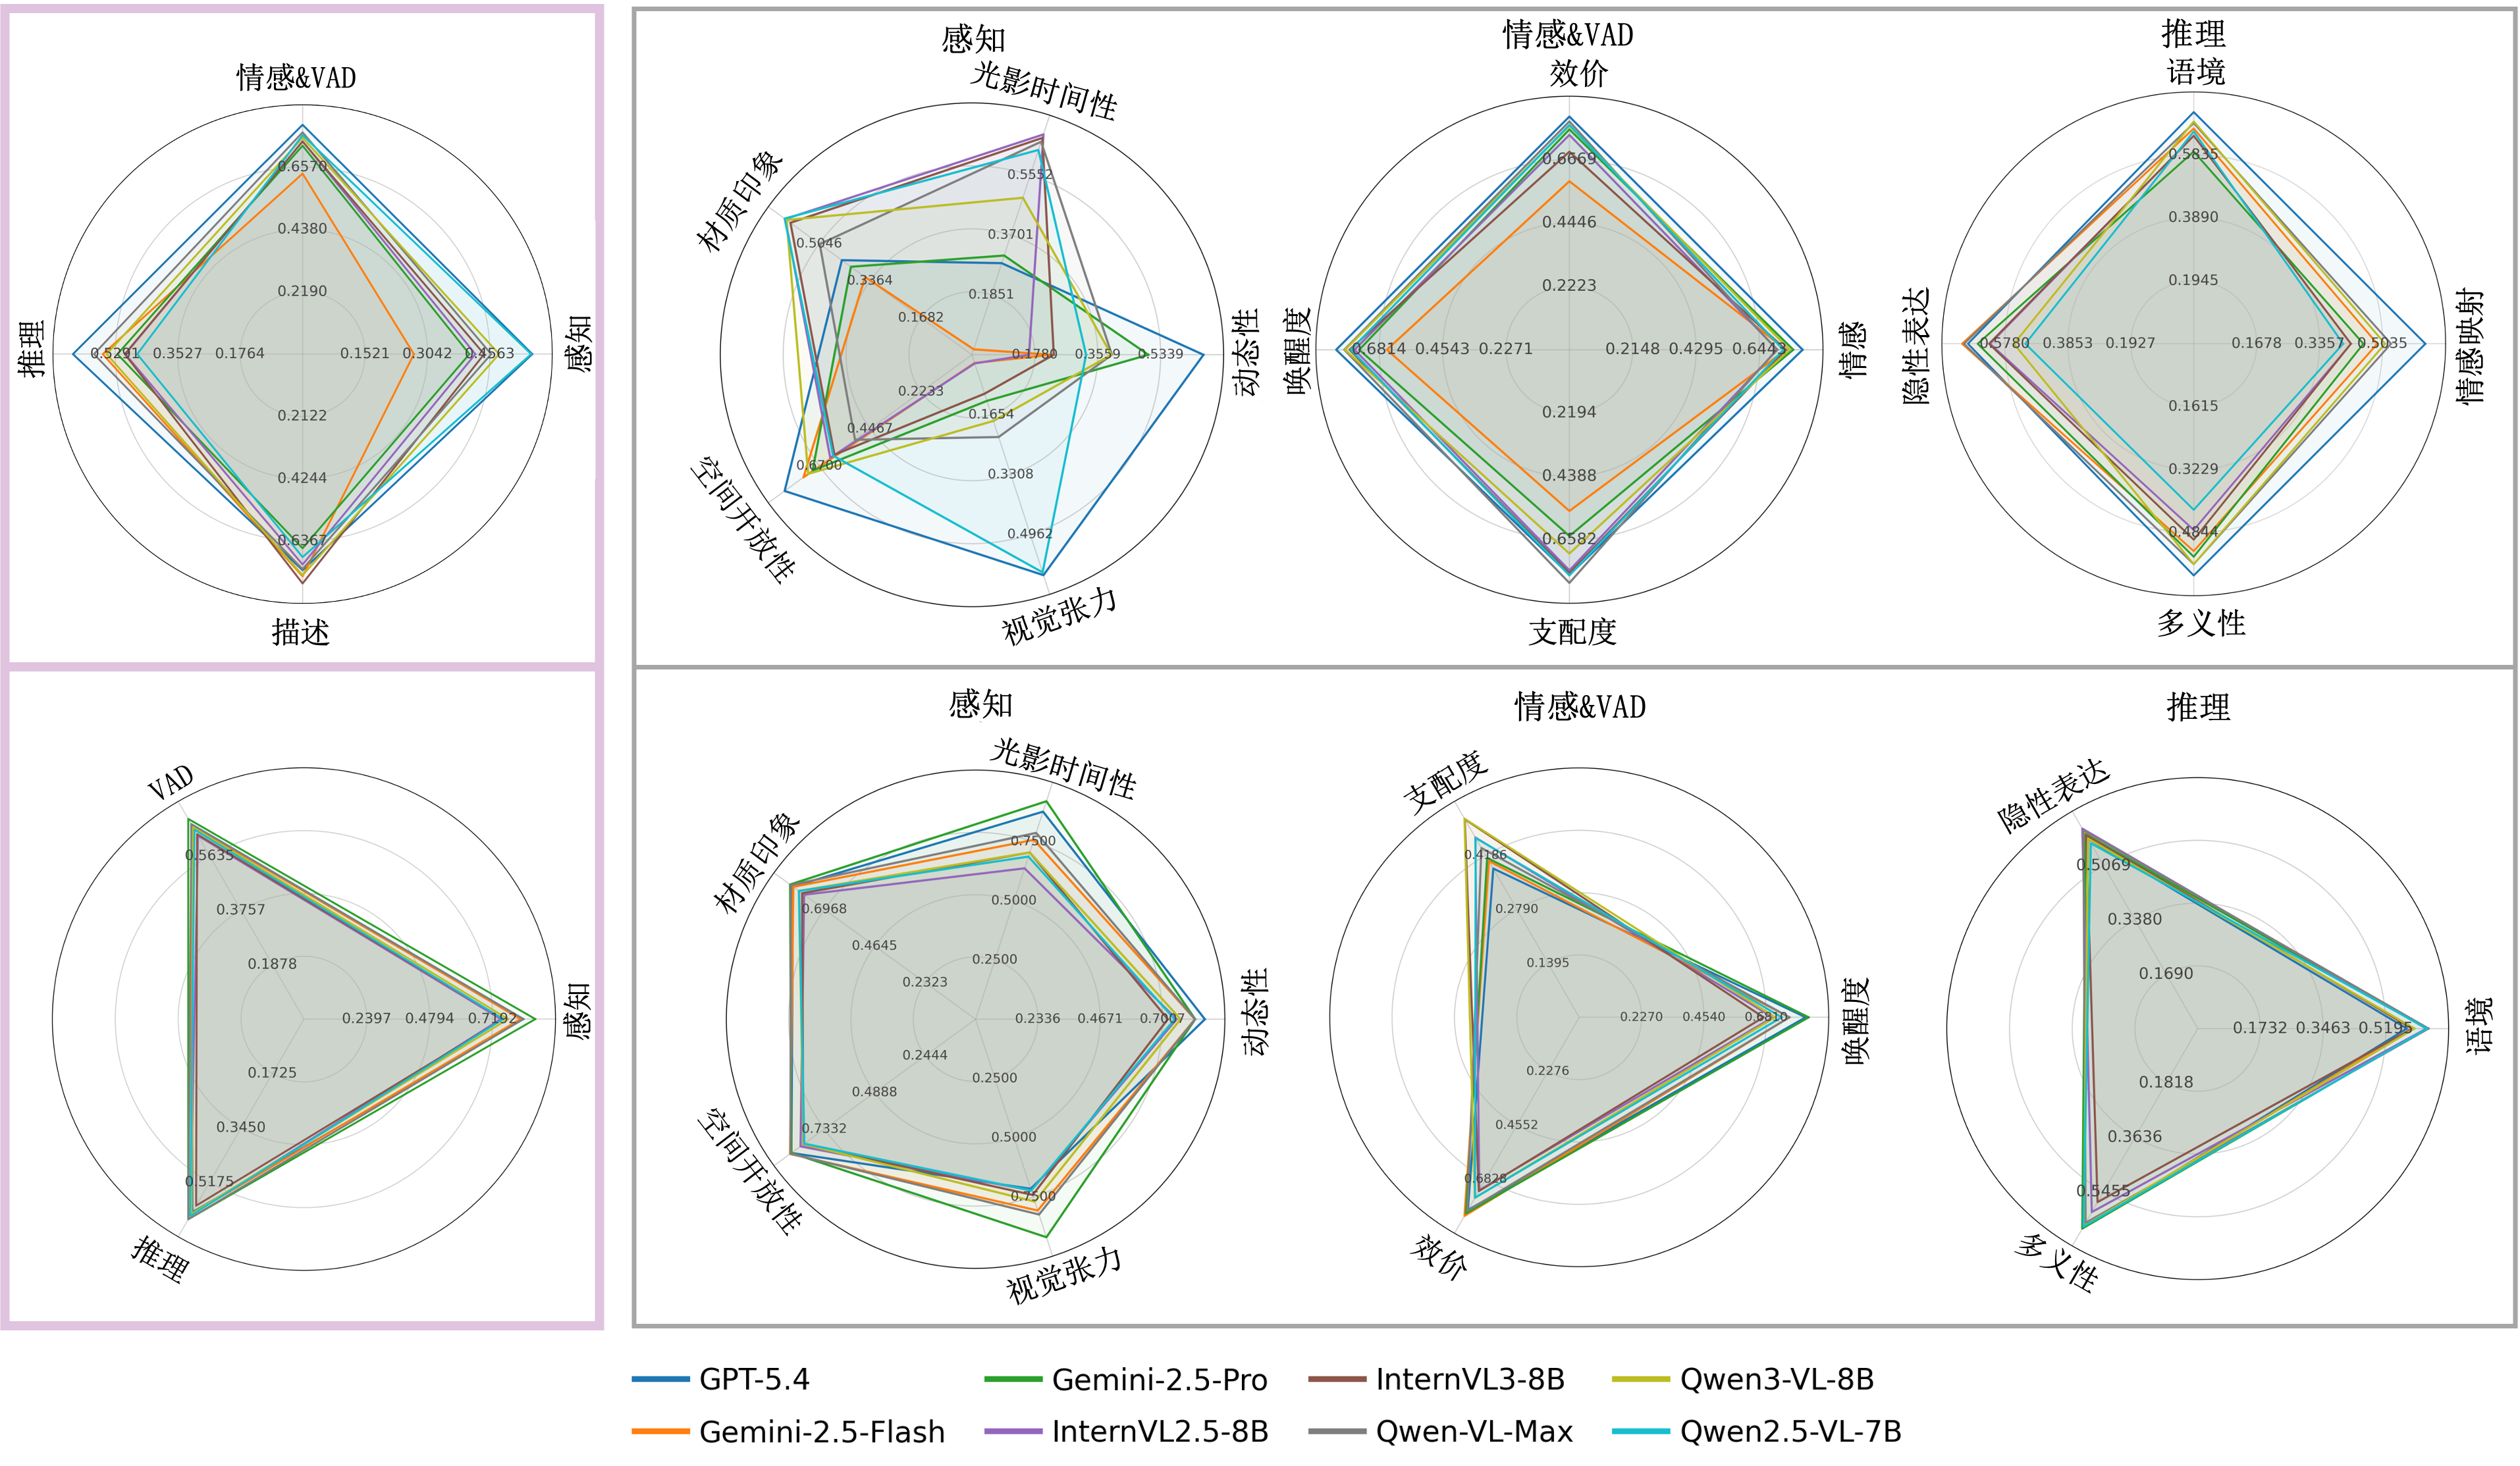
\includegraphics[width=0.95\textwidth]{figures/aerbench/radar_re.png}
    \bicaption[fig:chap5_radar]{}{代表性的8 个 MLLM 在单图与双图设置下的雷达图对比}{Fig.}{Radar plots for single-image (top row) and paired-image (bottom row) evaluations on eight representative models, including the top-4 closed-source and top-4 open-source MLLMs; the two plots on the left summarize core dimensions, while the six plots on the right show task-level performance per dimension}
\end{figure}



基于表~\ref{tab:chap5_main_results} 与图~\ref{fig:chap5_radar} 的系统评测结果，本节提炼出四项贯穿任务族与模型设置的核心发现，分别对应“感知—情感—推理”三级能力上的不同失效模式。

\begin{itemize}
\item 发现 1：情感标签比感知机制更容易。单图评测结果显示，情感与 VAD 预测在所有模型上都是表现最稳定的任务族：GPT-5.4 取得最高分 0.8760，Qwen-VL-Max 取得 0.8472，Qwen2.5-VL-7B 取得 0.8364，Qwen3-VL-8B 取得 0.8265。这说明 MLLM 已经能够相当可靠地识别作品的粗粒度情感倾向，并将作品映射到离散或连续的代表性情感表征。然而这一优势并未直接迁移到感知维度识别。即使是表现最佳的模型 GPT-5.4 与 Qwen2.5-VL-7B 在感知任务上也仅取得 0.6084 与 0.6054。图~\ref{fig:chap5_radar}（上行）进一步显示，模型在材质印象、空间开放性与光照时间性上的表现相对较好，而在动态性与视觉张力上的离散度显著更大。这一模式说明：静态或表层线索较易识别，而涉及“隐含运动、构图张力”等更专业的视觉属性则需要更专门的感知敏感度。因此，高情感/VAD 准确率不应被解读为完整的艺术理解：模型可能在不准确识别“支撑情感判断的感知机制”的情况下输出看似合理的情感状态。

\item 发现 2：流畅描述不保证基于证据的推理。 推理与描述任务揭示了模型能力上的互补短板。GPT-5.4 在单图推理上领先，Qwen-VL-Max 与 Gemini-2.5-Pro 紧随其后。情感/VAD 与推理之间的分数差表明：模型虽然常常能够给出看似合理的情感标签，但难以将这些标签构建为忠实于视觉证据、上下文线索与表达模式的解释。描述任务则呈现不同模式：Gemini-2.5-Flash 取得最高分 0.8226，Qwen3-VL-8B 也取得 0.8185，超过 GPT-5.4 的 0.8000。这说明流畅的情感化描述更多受益于通用生成能力与视觉摘要能力，而严格的推理要求更精确地将“声明”与“证据”对齐。推理雷达图（图~\ref{fig:chap5_radar} 上行右侧）进一步揭示了这一局限：上下文类推理相对较强，而感知—情感映射与歧义消解类推理仍显著薄弱。换言之，模型更擅长生成连贯的情感语言，而非解释“作品为何引发特定情感反应”。

\item 发现 3：对比有助于感知但无助于情感校准。双图评测为情感比较判断提供了独立测试。Gemini-2.5-Pro 在双图整体性能上取得最高分，其后依次为 Qwen-VL-Max、GPT-5.4、Gemini-2.5-Flash、Qwen3-VL-8B。相较于单图任务，头部模型在配对感知上的得分普遍提升——Gemini-2.5-Pro 达到 0.9589，GPT-5.4 达到 0.9100。这表明相对比较能够使显著的感知差异更易检出，尤其当两件作品在张力、空间开放性、运动或光照上形成直接对比时。但双图评测也暴露出情感校准上的持续困难：Gemini-2.5-Pro 取得最高 0.7514，开源模型中 Qwen3-VL-8B 取得 0.7200，但仍有多个模型得分低于 0.55。雷达图（图~\ref{fig:chap5_radar} 下行）也显示 Gemini-2.5-Flash 与 Gemini-2.5-Pro 在单图感知上偏弱，但在配对任务上表现强劲。这一对比表明 Gemini 系列更擅长识别“相对情感差异”，而在为单件作品赋予“绝对感知标签”时能力相对受限。因此，双图设置以测试关系型情感判断补充了单图评测，避免了模型仅依赖图像内在先验。

\begin{figure}[!htbp]
    \centering
    \subfigure[]{
        \includegraphics[width=0.95\textwidth]{papers/AER-Bench/figures/cases.pdf}
    }
    \hfill
    \subfigure[]{
        \includegraphics[width=0.95\textwidth]{papers/AER-Bench/figures/description_case.pdf}
        }
    \bicaption[fig:chap5_cases]{}{（a）推理与（b）描述任务的成功与失败定性案例}{Fig.}{Qualitative cases of success and failure patterns in affective reasoning and description. (a) reasoning cases; (b) description cases}
\end{figure}

\item 发现 4：主要瓶颈是基于证据的解释。 跨任务族来看，最强表现集中在情感/VAD 与配对感知上，而最大短板则出现在精细化感知与推理上。这一非对称性表明：当前 MLLM 更擅长给出“看似合理的情感标签或描述”，但在识别“支撑这些标签的中介感知机制”上仍存在系统性差距。上述结果支撑了 AER-Bench 的诊断动机：艺术情感理解不应仅以“模型是否预测出正确情感”作为评价基准，而应同时考察模型能否（1）识别相关的美学线索、（2）比较作品之间的情感差异、（3）将自身的解释组织为“基于证据的、有逻辑的陈述”。本基准因此揭示了当前 MLLM 的核心能力缺口：它们能够流畅地“谈论”情感，却仍难以将情感主张锚定到精确的视觉与上下文证据之上。
\end{itemize}

% \FloatBarrier

% \subsection{定性案例与经验启示}

% \label{sec:chap5_cases_insights}

图~\ref{fig:chap5_cases} 给出了 AER-Bench 推理与描述任务的代表性定性案例。推理案例覆盖了四类核心推理——上下文解释、情感歧义、表达模式、感知—情感映射——并不仅检验模型是否给出“看似合理的情感”，还检验其能否将视觉证据、上下文线索与情感概念整合为连贯的解释。描述案例进一步显示“流畅语言”不足以支撑可靠的情感理解：模型虽然生成了“冲突”“神秘”“荒凉”等看似贴切的情感短语，但遗漏或错位了若干关键视觉证据，包括锯齿状的线条、暗沉的色调、壕沟般的阻断、铁丝网般的形态、粗糙的肌理与压迫感的天空。与参考标注相比，模型输出抓住了“氛围片段”却未能将其组织为对 alarm、tension、frustration、entrapment、hostility、历史性创伤等情感的忠实证词支撑。

上述统计画像与多维发现共同指向三点核心启示。其一，从统计层面看，AER-Bench 在标签空间多样性、情感—VAD 内部一致性、感知—情感关联强度上同时具备可解释性，模型既不能仅依赖情感标签的先验偏置取得高分，也不能仅依赖通用视觉语义绕过艺术特有的中介线索。其二，从能力层面看，当前 MLLM 存在“情感识别强—感知机制弱”、“流畅描述强—证据推理弱”、“配对感知强—情感校准弱”三组非对称短板，其中“基于证据的解释”是最为普遍的能力瓶颈。其三，从诊断价值看，AER-Bench 通过将失败模式定位到上下文锚定、歧义消解、表达模式判断、感知—情感映射与描述综合等多个环节，能够为后续模型迭代提供独立的优化目标。

% \subsection{本节小结}

% 本节从“统计画像—系统评测—核心发现—定性案例”四个层次，给出了 AER-Bench 的完整分析结果。统计层面，基准在情感偏态分布、情感—VAD 内部一致性（$\epsilon^2 \geq 0.293$）与感知—情感共现结构（视觉张力 $V=0.5310$）上同时具备多样性、可解释性与诊断性；评测层面，14 个代表性 MLLM 在 AER-Bench 上的整体能力可被清晰刻画为“情感识别相对成熟、感知机制与证据推理显著薄弱”的能力非对称结构；发现层面，四项核心发现分别揭示了情感—感知的不对称、流畅—证据的不对称、相对—绝对判断的不对称以及“基于证据的解释”这一主要瓶颈；案例层面，定性证据进一步表明基准能够将“表层情感流畅”与“基于证据的解释”清晰区分，从而为后续艺术场景下的可解释视觉基础模型研究提供可扩展的诊断平台与改进方向。
\FloatBarrier

\section{本章小结}

本章围绕多模态大语言模型在艺术情感理解上的能力边界，构建了层级化任务体系与统一评测协议。在任务设计上，将艺术情感理解拆解为感知、情感、推理与描述四个互补层级，并将每一层级实例化为可重复生成的评测题目；在评测协议上，借助生成式模型辅助的结构化标注、相似度过滤与人工核验，并结合确定性度量和基于评分细则的语义评判，覆盖单图与配对两种设置。对 14 个代表性多模态大语言模型的系统评测表明，模型能够给出较可靠的情感判断或流畅描述，但基于视觉证据的解释仍是突出短板。与前文通过适应和先验融合提升跨域、跨类别迁移能力不同，本章不更新被评测模型，而是评估其面对更高层级语义任务时的能力适用范围，为后续模型迁移与优化明确可检验的目标。

% Local Variables:% Local Variables:
% TeX-master: "../thesis"
% TeX-engine: xetex
% End:
